\subsection{Experimental Evaluation}
To evaluate the proposed approach and show the feasibility of enabling existing TCP-based applications to perform seamless handovers, we performed extensive emulations in two scenarios.
% In this section, we present the experimental environment and discuss the evaluation results.


\begin{figure*}[tb]
    \centering
    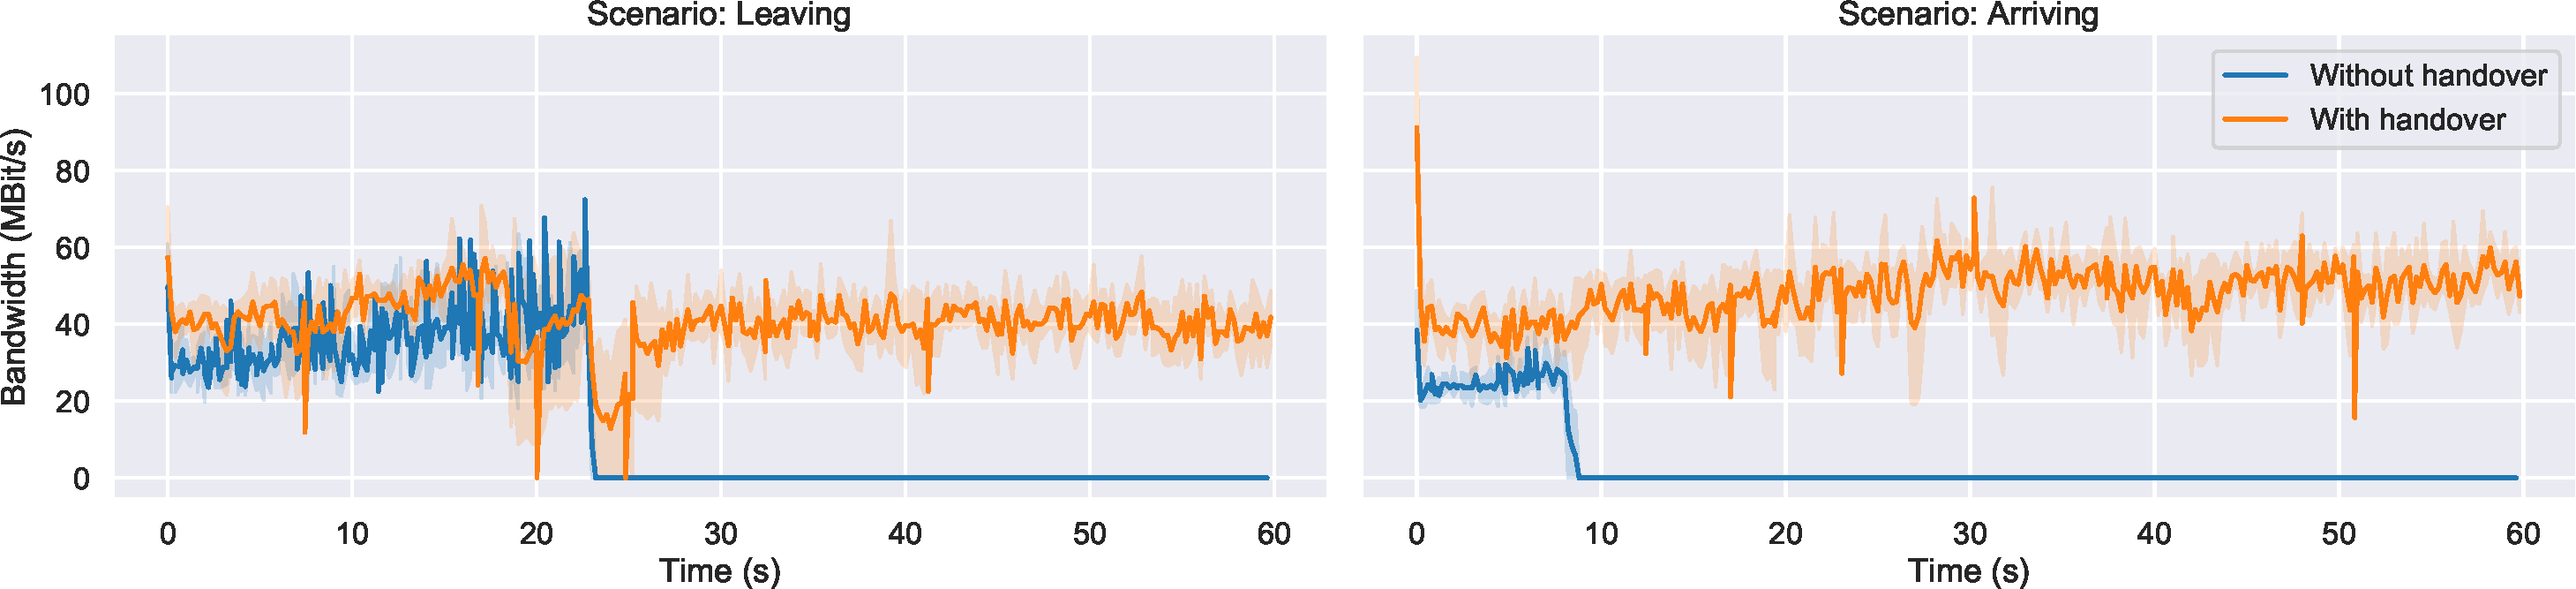
\includegraphics[width=\textwidth]{figures/migration/wg_migration-network.pdf}
    \caption{Network throughput with and without connection migration for two scenarios}
    \label{fig:eval:mig:network}
\end{figure*}
\begin{figure*}[tb]
    \centering
    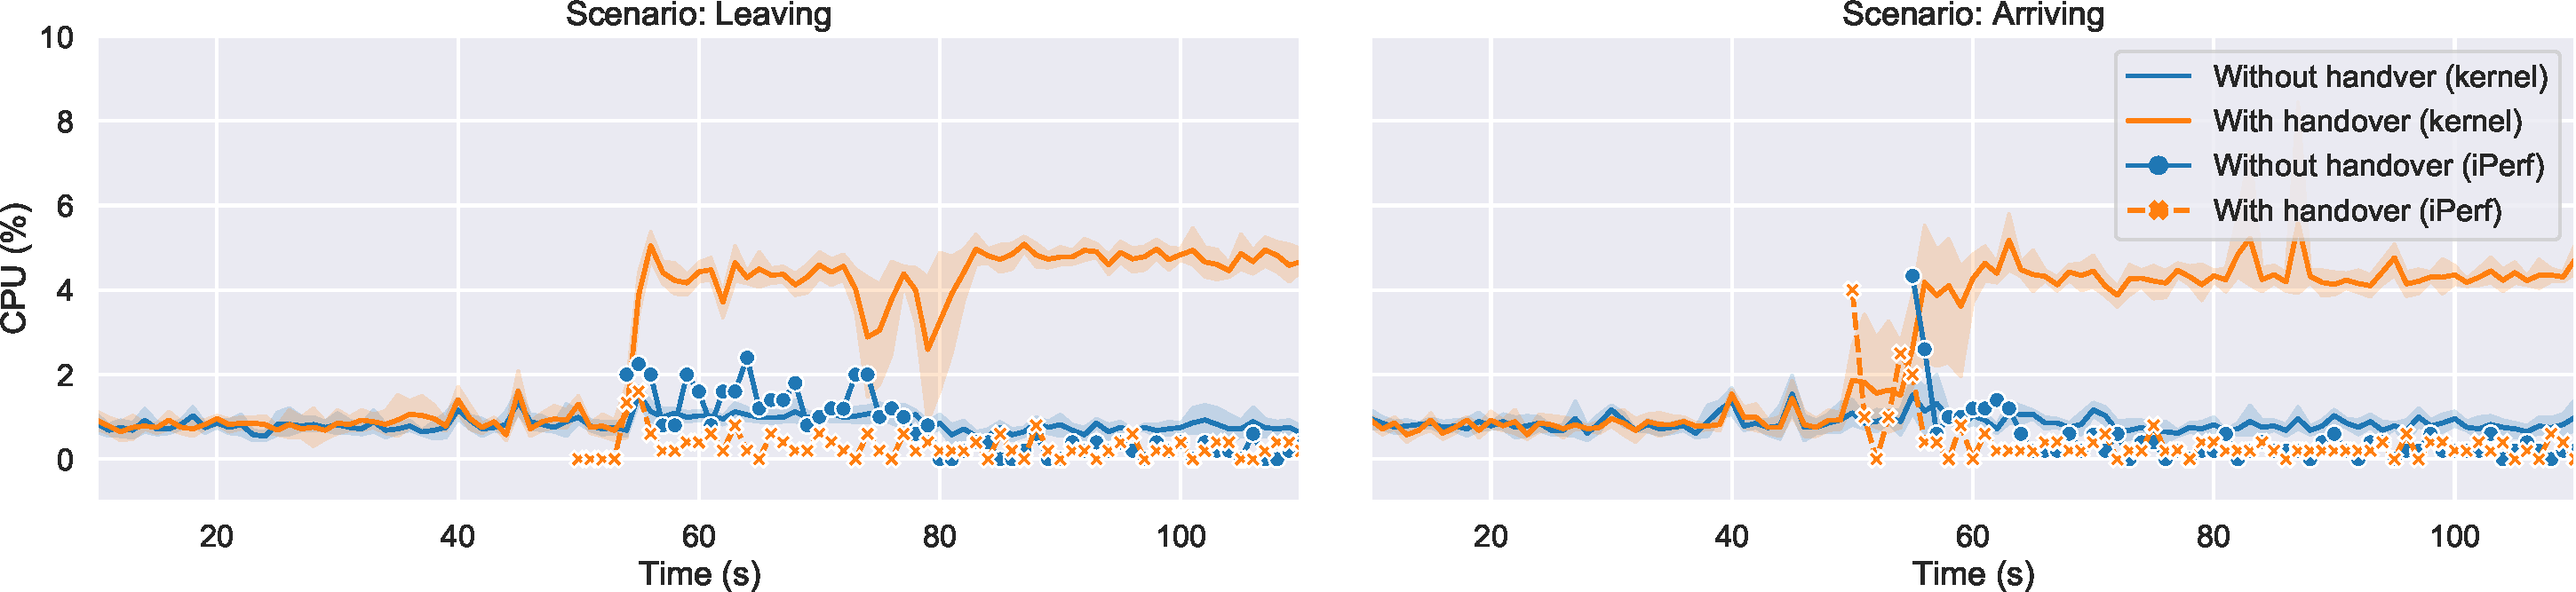
\includegraphics[width=\textwidth]{figures/migration/wg_migration-cpu.pdf}
    \caption{CPU usage with and without connection migration for two scenarios}
    \label{fig:eval:mig:cpu}
\end{figure*}


\subsubsection{Experiment Setup}
% \paragraph{Emulation}
To conduct the evaluation, two scenarios were emulated, of which the first one (S1) simulates leaving a location.
Here, the handover is performed from Wi-Fi to LTE.
The second scenario (S2) simulates the corresponding handover from LTE to Wi-Fi, e.g., when entering a building providing a Wi-Fi connection.
In order to perform these experiments, the \emph{Common Open Research Emulator (CORE)}\footnote{\url{https://coreemu.github.io}} was used, that allows execution of arbitrary programs.

\begin{figure}[ht]
    \centering
    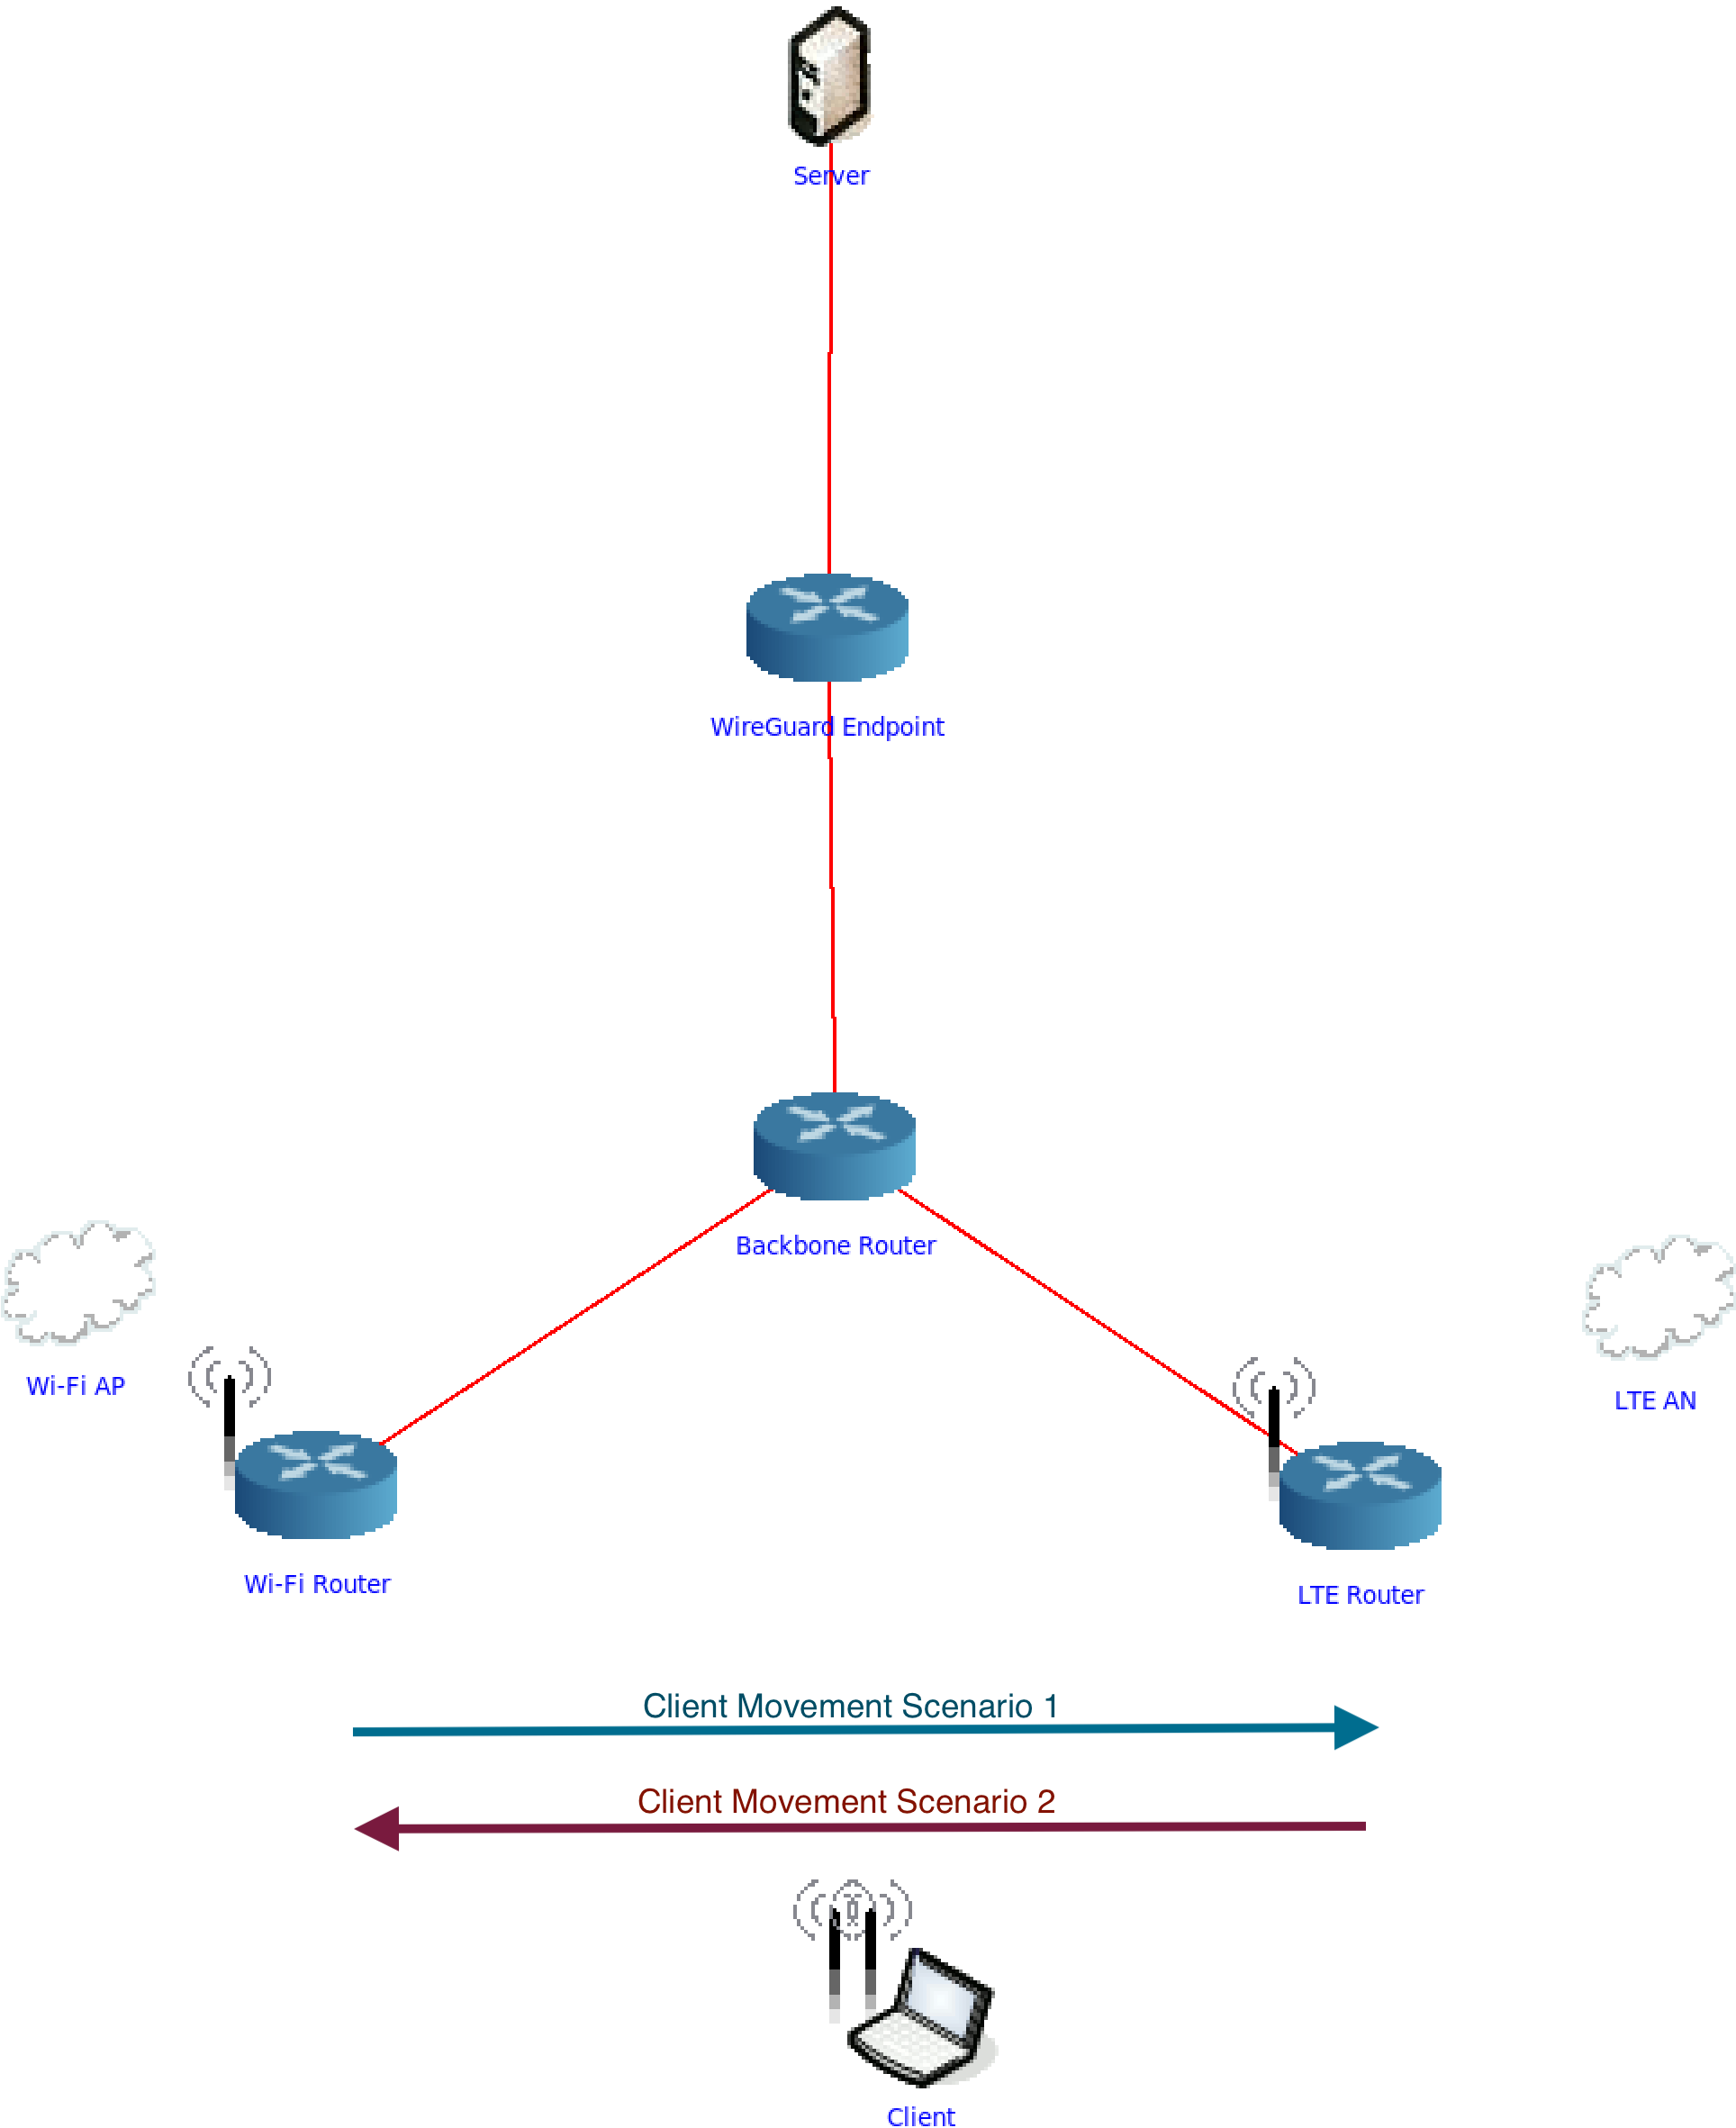
\includegraphics[width=.9\columnwidth]{figures/migration/topo.png}
    \caption{Simulated topology used for the evaluation}
    \label{fig:eval:mig:topo}
\end{figure}

% \paragraph{Topology}
Fig.~\ref{fig:eval:mig:topo} shows the topology used for the evaluation.
% Within the emulation, the following nodes were modeled.
% First, a mobile client node is required, which is the bottom node in Fig.~\ref{fig:eval:mig:topo}.
The client (bottom) contains the TCP-based application that shall be enabled with handover capabilities and the WireGuard client.
Further, the client node is the only node moving throughout the emulation.
In S1, the client moves from left to right (blue arrow) and loses the Wi-Fi connection roughly in the middle of the movement range. 
In S2, the node moves from right to left (red arrow) and regains the Wi-Fi connection at the same position.
The LTE connection is available throughout the entire experiment, whereby the Wi-Fi connection is prioritized if available.
The mobility is modeled in a way to simulate human walking, i.e., 5 to 6 km/h.
Further, we modeled a Wi-Fi access point (Wi-Fi AP on the left) and a corresponding Wi-Fi router.
% The client is connected to the Wi-Fi AP, which in turn uses the Wi-Fi router to route traffic.
We modeled the Wi-Fi AP to match the IEEE 802.11ac standard, i.e., roughly 1 Gbit/s throughput.
On the bottom right in Fig.~\ref{fig:eval:mig:topo}, the LTE access network (LTE AN) was modeled to match current LTE speeds of about 100 MBit/s.
% The LTE AN is connected to a LTE router.
In the middle of the topology, a router was modeled to mimic the backbone of the network, i.e., the network of an ISP connecting multiple parts of the Internet.
The second node from the top is the WireGuard endpoint, that is used to terminate the WireGuard tunnel.
% From this node, the arriving encapsulated TCP connection from the client is extracted and relayed to the server and TCP-packets from the server encapsulated and transmitted using WireGuard to the client.
% The WireGuard endpoint node also acts as a regular backbone router in experiments not using the WireGuard tunnel.
Finally, the server node is modeled (top), which only contains the application's server.

% The red connections in Fig.~\ref{fig:eval:mig:topo} represent wired connections between the corresponding nodes.
% The connection between the Wi-Fi router and the backbone router is modeled to mimic a standard uplink that can be found in homes with 100 MBit/s.
% The other wired connections are using links of multiple GBit/s, which are however not relevant as the limiting links are the LTE AN connection and the connection between the Wi-Fi router and backbone router.

% \paragraph{Applications}
In order to simulate a TCP-based application, iPerf3\footnote{\url{https://iperf.fr}} was used.
iPerf3 is an open-source tool for measuring network throughput in IP network following the client-server paradigm and supports various transport layer protocols.
% The server node in the evaluation topology runs an iPerf3 server, whereas the client node runs the iPerf3 client.
The client initiates the connection to the server upon experiment start using the currently active connection, i.e., Wi-Fi if available, otherwise LTE.
Each experiment was executed for 120 seconds in total.
Within the first 50 seconds, where used to allow the emulation establish routes throughout the network, so that packets can be routed from client to server and back again.
As soon as the routes were announced, the movement and iPerf started for 60 seconds.
The last 10 seconds were used to tear down the emulation.
In addition to the presented handover-approach, we also conducted experiments without a tunnel, using the regular routing mechanisms of the Linux kernel to be able to compare the achievements of our approach.
Each experiment was repeated five times to reduce effects like race conditions during booting the emulation and other side effects.

\subsubsection{Results}

% \paragraph{Supporting Vertical Handovers}
Fig.~\ref{fig:eval:mig:network} shows the results for the conducted experiments.
The x-axis denotes the experiment time, while the y-axis denotes the achieved bandwidth.
The left sub-plot visualizes the leaving scenario, while the right sub-plot visualizes the arriving scenario.
Finally, the orange graphs show experiments, where the proposed handover mechanism is enabled, the blue graphs show the results without employing the WireGuard tunnel for comparison.
As can be seen in both scenarios, the proposed approach for using WireGuard to enable TCP-based applications with vertical handover capabilities, works  as proposed.
Especially in the arriving scenario, the throughput of the iPerf application does not drop at all.
Without the WireGuard tunnel, throughput decreases because the iPerf or, in particular, the TCP connection is not re-established after the connection is changed.
In the leaving scenario, a small drop is visible at around 25 seconds.
This is due to the fact that the Wi-Fi connection is lost immediately, resulting in a short connection drop until he kernel recognizes the lost connection and propagates the changes to the routing tables.
In the arriving scenario, however, this drop is not visible since the LTE connection does not break but rather the Wi-Fi connection is established in parallel.
As soon as the kernel detects the new Wi-Fi connection, the WireGuard tunnel uses the Wi-Fi connection, whereas in the blue graph it is visible, that, although the LTE connection is still available, the TCP connection does not continue due to the newly established Wi-Fi connection.

% \paragraph{Overhead Analysis}
Although the handover capabilities offer a great improvement for users, the WireGuard tunnel introduces some kind of overhead because it has to encapsulate the TCP-connection and introduces encryption.
To quantify this overhead, the CPU usage of both the kernel and the iPerf process was monitored, which can be seen in Fig.~\ref{fig:eval:mig:cpu}.
Fig.~\ref{fig:eval:mig:cpu} is composed the same way as Fig.~\ref{fig:eval:mig:network}.
The y-axis, however, denotes the CPU utilization of the client node.
Further, the solid graphs show the kernel's CPU usage, while the graphs with markers show the CPU utilization of iPerf.
First, the iPerf CPU usage does not differ significantly, regardless of the scenario and whether the WireGuard based handover mechanism is used.
The kernel, however, shows quite a different result.
On the one hand, the blue graphs, i.e., without the WireGuard tunnel, show that the kernel's CPU utilization is relatively constant at around 1\% for the entire experiment.
In the orange graphs, on the other hand, show an increase of CPU utilization of around 3\% as soon as iPerf starts sending data, which is the same for both scenarios.
The two drops in the leaving scenario around the 80 seconds mark align with the network drop visible in Figure~\ref{fig:eval:mig:network}, where iPerf is not able to send data for the time of the handover.

Considering the improvement in the users' connection with consistently high network quality using our method, only 3\% of additional CPU consumption is an acceptable overhead.
Moreover, iPerf specifically tries to make maximum use of the available bandwidth.
For applications that have a normal usage profile, it is to expect that the overhead will be significantly lower.
Finally, the authors have shown in past work how to reliably predict Wi-Fi connection loss~\cite{hochst2019learning}.
Thus, a system that only activates the WireGuard tunnel when a connection loss is expected is conceivable, which would limit the CPU utilization overhead to a few seconds in time.
